%!TEX root = ../main.tex

\chapter{Performance and optimization}
\label{chp:performance}
\noindent
Running a \ac{VR} application is highly resource-intensive. Not only must the processor handle all sensor data, but it also has to run a 3D application that is rendered on two screens, aiming to achieve at least a stable 72 \ac{FPS} experience.
On top of that, the Meta Quest 2 has limited mobile hardware Tab.[\ref{tab:specs}]. This chapter will explain all the optimizations necessary to run the application at 90 \ac{FPS}, as well as demonstrate the performance of the OBJ parser build.


\begin{table}
  \centering
  \begin{tblr}{
      colspec = {|l|l|},
      rows={valign=m},
      row{1}={font=\bfseries}
    }
  \hline
  Charateristic & Specs                                                          \\ \hline
  Chipset       & Qualcomm Snapdragon XR2                                       \\ \hline
  CPU           & Octa-core Kryo 585 (1$\times$2.84 GHz, 3$\times$2.42 GHz, 4$\times$1.8 GHz)  \\ \hline
  GPU           & Adreno 650                                                    \\ \hline
  RAM           & 6 GB LPDDR5                                                    \\ \hline

  \end{tblr}
  \caption{Meta Quest 2 specs}
  \label{tab:specs}
\end{table}

\section{Meta XR performance check}
\noindent
Thanks to the Meta XR plugin, Meta directly suggests certain options to enable or disable. The most important aspects will be explained in the next paragraphs.

\paragraph{Post-processing}
must be disabled because it can be very demanding on the device. As discussed in Chapter \ref{Chp:fade}, mobile HDR is already turned off, however, \ac{UE} still enables lens flares by default. 
To disable it, we need to place a \texttt{Post Process Volume} in the scene and set the lens flare intensity to \texttt{0}.

\paragraph{Dynamic lighting}
must be disabled. This option is probably the most impactful. When enabled, the app runs at less than 60 \ac{FPS}, but with it disabled, performance reaches a stable 90 \ac{FPS}, yielding an improvement of over 30 \ac{FPS} and providing a more stable experience overall.
Unfortunately, dynamic lights can enhance immersion, however, the only moving elements are the \texttt{VR Characters} and the \texttt{3D Model Viewer}, so the absence of dynamic lighting will not be very noticeable.\\
Static lighting will still be used, allowing the environment to have shadows cast by a directional light that simulates the sun, as well as by rectangular and point lights used for building interiors.

\paragraph{Half precision float for materials and shaders.}
As is well known, using smaller float values can improve system performance by sacrificing some precision, though fortunately, the side effects are often negligible.
However, in our case, this optimization has limited impact because the majority of materials used are static.

\subsection{Other optimizations for Meta quest}
\noindent
In addition to the previously described options, there are some additional settings that can help boost performance. These are simple Android manifest tags that enable the \ac{HMD} to activate additional functionality:

\begin{itemize}
  \item \textbf{Suggested CPU and GPU levels:} This setting allows the \ac{HMD} to operate at maximum performance levels.
  \item \textbf{Processor favor:} This option lets us choose whether the \ac{HMD} should prioritize maximum performance for either the GPU or CPU. This is useful because the device has limited power and heat dissipation, preventing it from running at 100\% performance continuously without the risk of throttling.
  \item \textbf{Enable dual core:} Normally, the \ac{HMD} uses only one core for the foreground app, but a meta tag enables a second core for background activities and parallel operations. This is particularly beneficial for the parser and asynchronous operations needed by \ac{UE}.
\end{itemize}

\section{Optimizations for Unreal engine VR}
\noindent
In addition to the options provided by the Meta XR performance check, there are settings within \ac{UE} (Bib.\cite{UEperformance}) that can further optimize the app for the \ac{HMD}.These optimizations are explained in the following paragraphs.

\paragraph{Instanced stereo}
When rendering a frame for an \ac{HMD}, the screens are typically managed as two separate entities. This is demanding for the GPU, as it has to render two frames simultaneously.
However, with Instanced Stereo, we can generate both views in a single pass. \ac{UE} achieves this by applying a small transformation to the loaded vertices, correcting the view difference between the left and right eyes. Additionally, this transformation is applied to shaders as well.
This rendering method relies on low-level \ac{API}s that enable it, the Meta Quest 2 uses the Vulkan graphics \ac{API}, which supports this feature.

\subsection{Variable Rate Shading and Fixed Foveated Rendering}
\noindent
We don't always need to shade each material with maximum precision, so \ac{UE} provides tools to help mitigate this.

\paragraph{\ac{VRS}}
is a technique allows shaders to render at a lower resolution in specific situations.
Normally, the standard shading rate is 1:1, meaning one pixel shader invocation corresponds to one pixel target on the screen.
\ac{UE} offers various shading rates, for instance, applying a shading rate of 2x2 means that a single shader invocation will cover a 2x2 pixel area, resulting in one shading calculation for every 4 pixels.

\paragraph{\ac{FFR}}
is a technique that utilizes \ac{VRS} to determine which parts of the screen can be rendered at a lower resolution.
Studies, such as Bib.\cite{eye}, have shown that when viewing a screen, the eye typically focuses on the center.
This allows for lower resolution rendering in the peripheral areas. Consequently, as the distance from the center increases, we can apply a lower shading rate, conserving resources without noticeably impacting visual quality.\\
An example of \ac{FFR} zones is in Fig.[\ref{fig:FFR}] where the darker blue represents the lowest rate shading zone.


\begin{figure}[ht]
  \centering
  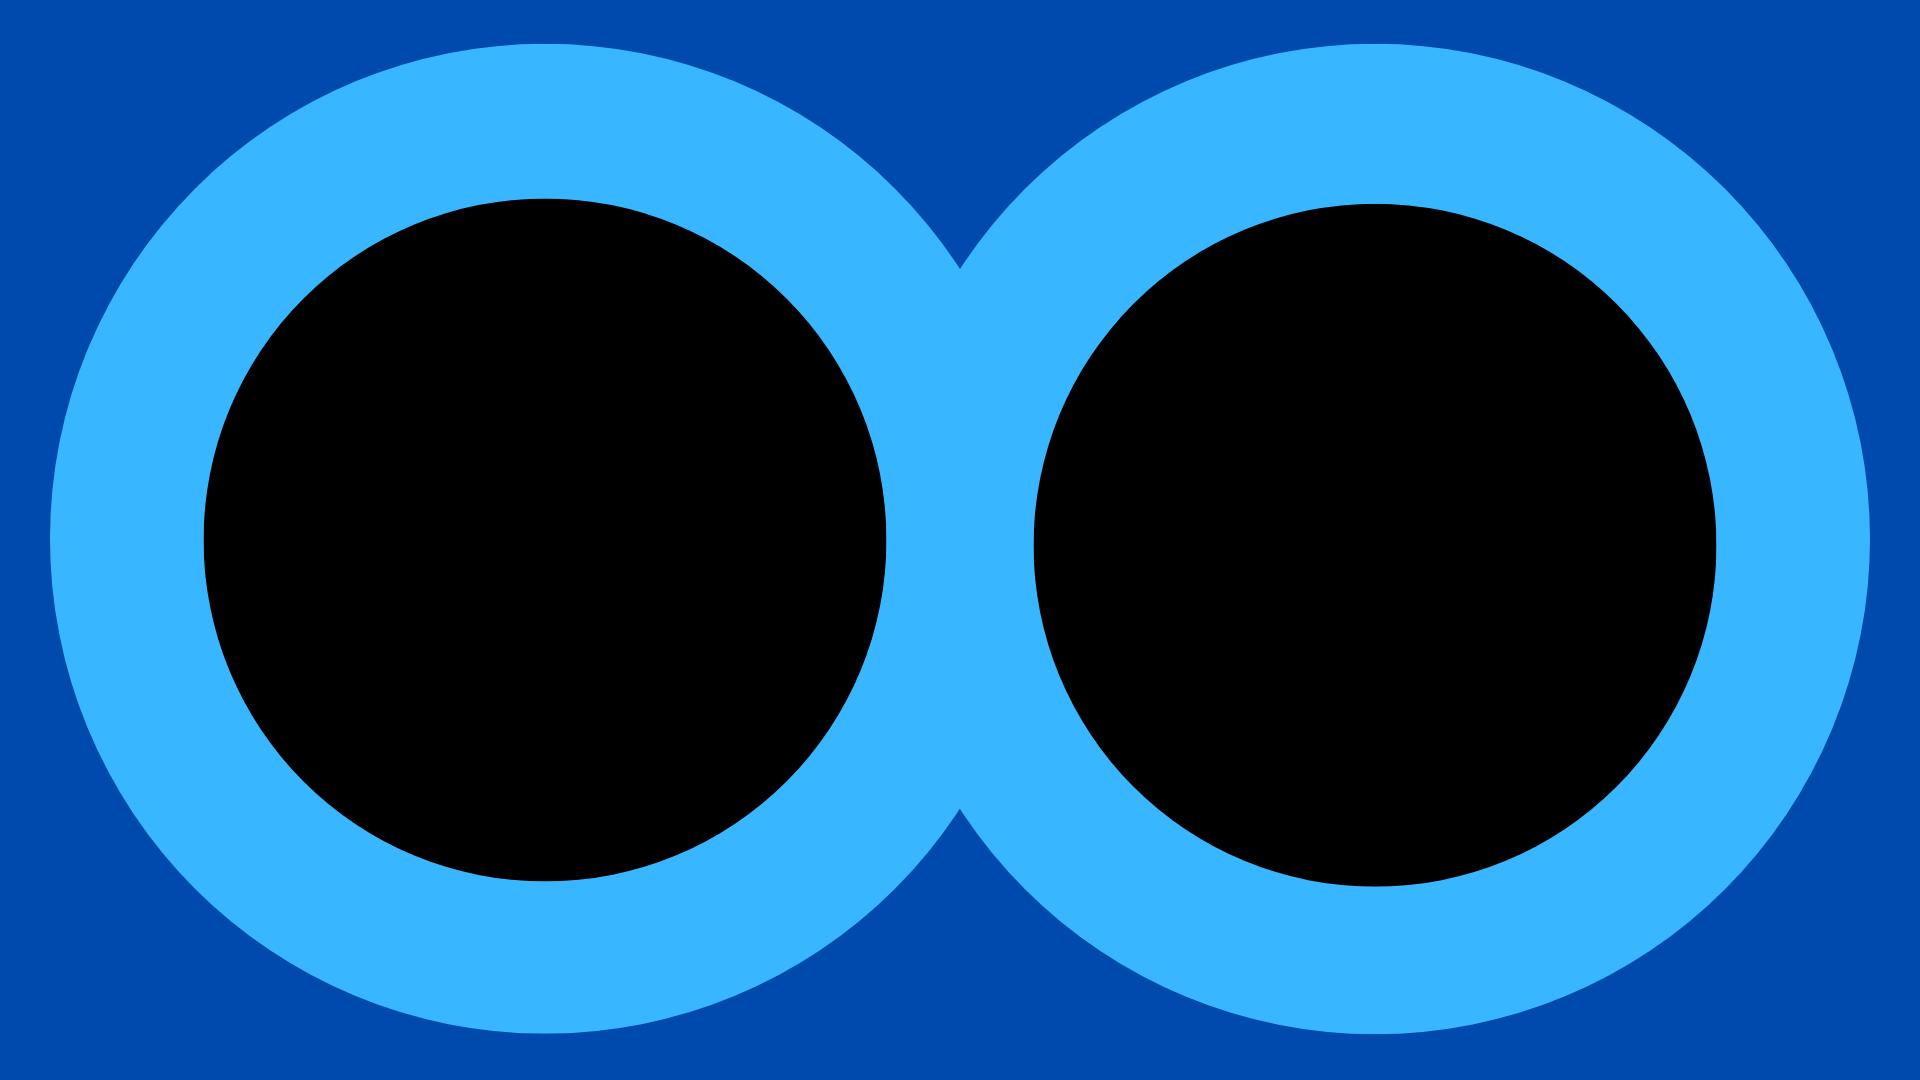
\includegraphics[width =0.96\textwidth]{FFR.png}
  \caption{Example of FFR zones}
  \label{fig:FFR}
\end{figure}

\noindent
As expected, \ac{FFR} is not an optimal approach, as the eye occasionally shifts to the periphery of the \ac{HMD} display.
In the future, \ac{HMD}s are likely to be equipped with eye-tracking modules, allowing \ac{FFR} to be replaced by dynamic foveated rendering, which adjusts rendering zones based on where the user is looking.

\section{General engine optimizations}
\noindent
\ac{UE} is one of the most important game engines on the market, offering many standardized features to optimize various types of games.

\paragraph{\ac{LOD}}
were created to reduce the number of vertices and triangles in a scene.
The concept is straightforward: small or distant objects do not require as much detail as closer or larger ones. 
Based on their position and size in the scene, each mesh has different \ac{LOD} levels that load according to the scene's requirements.
\ac{LOD} levels can be generated programmatically or model by a 3D artist, naturally, manual creation leads to more accurate \ac{LOD}.\\
\ac{LOD}s can modify materials or reduce the number of triangles and vertices. An example of programmatically generated \ac{LOD}s that reduce polygon count can be found in Fig.[\ref{fig:lods}].

\captionsetup[subfigure]{labelformat=empty}
\begin{figure}[h]
  \centering
  \begin{subfigure}{0.24\textwidth}
      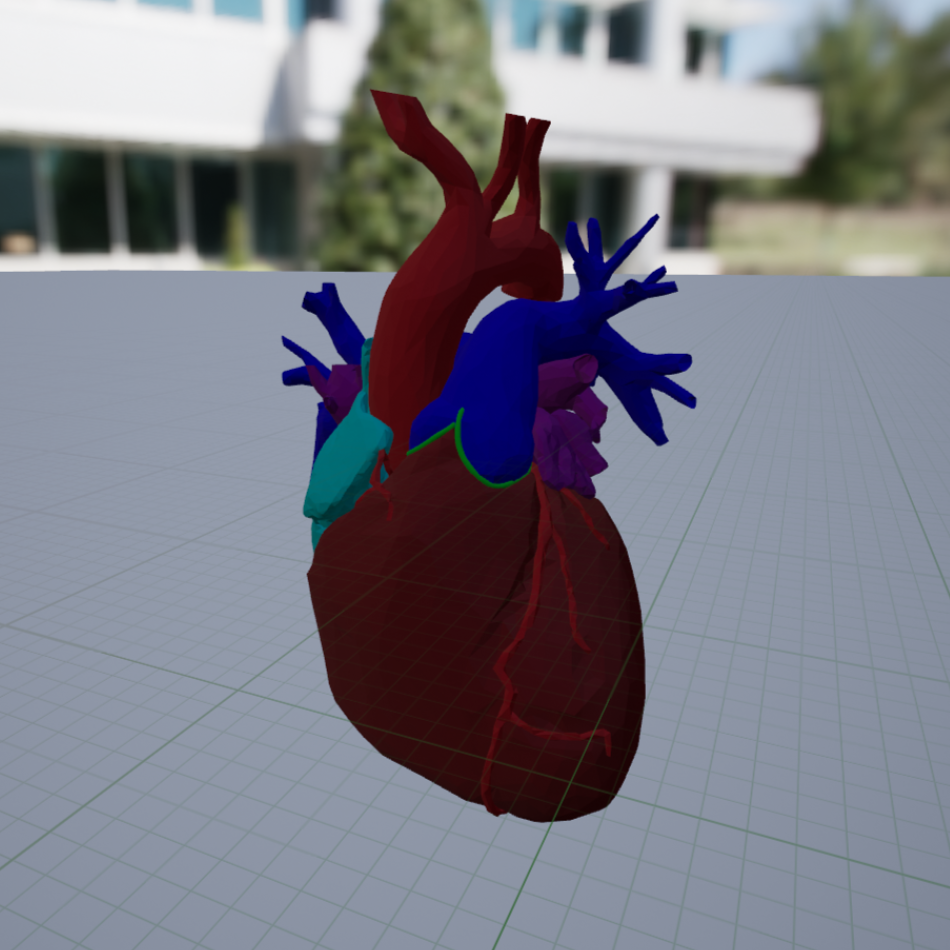
\includegraphics[width=\linewidth]{vrScreenshot/lod0.png}
      \caption{100\%}
  \end{subfigure}
  \begin{subfigure}{0.24\textwidth}
      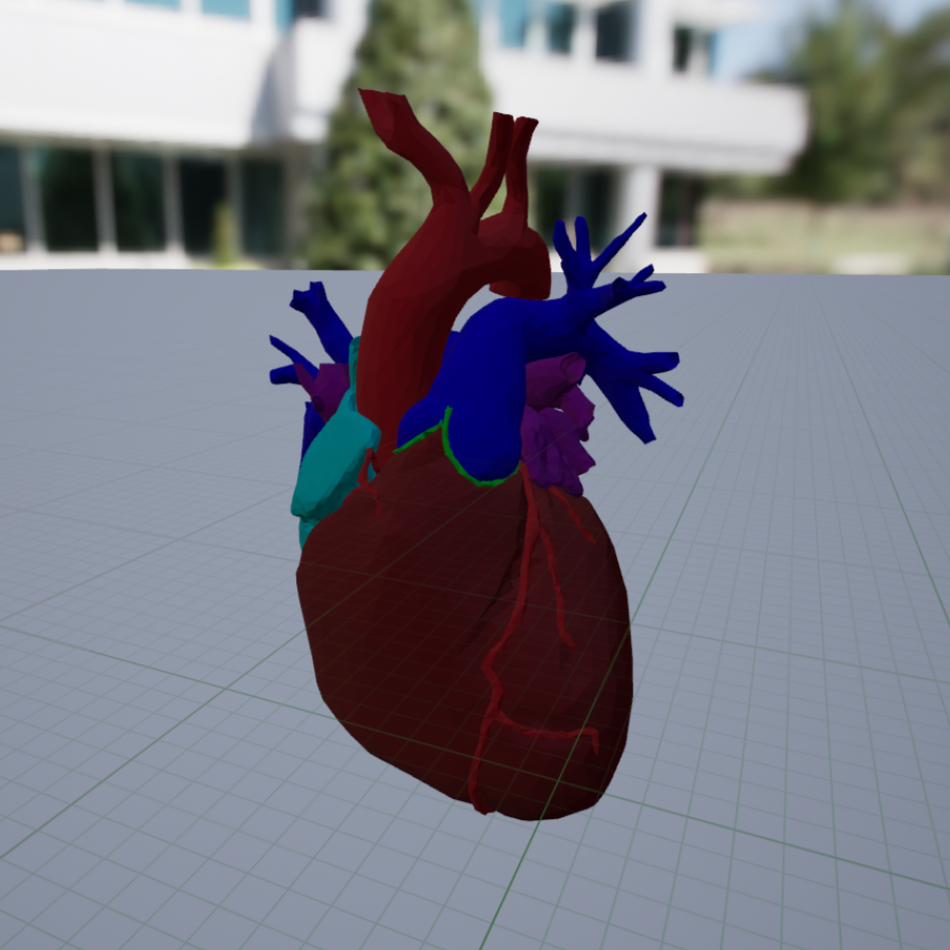
\includegraphics[width=\linewidth]{vrScreenshot/lod1.png}
      \caption{25\%}
  \end{subfigure}
  \begin{subfigure}{0.24\textwidth}
      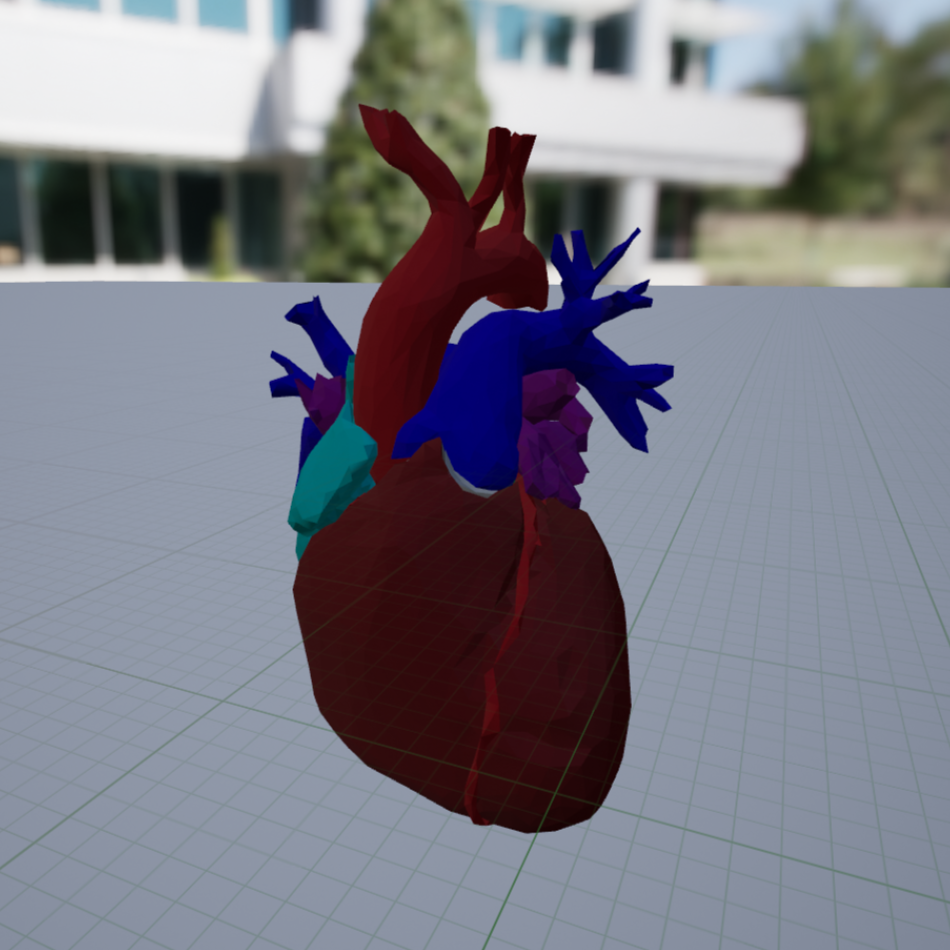
\includegraphics[width=\linewidth]{vrScreenshot/lod2.png}
      \caption{10\%}
  \end{subfigure}
  \begin{subfigure}{0.24\textwidth}
      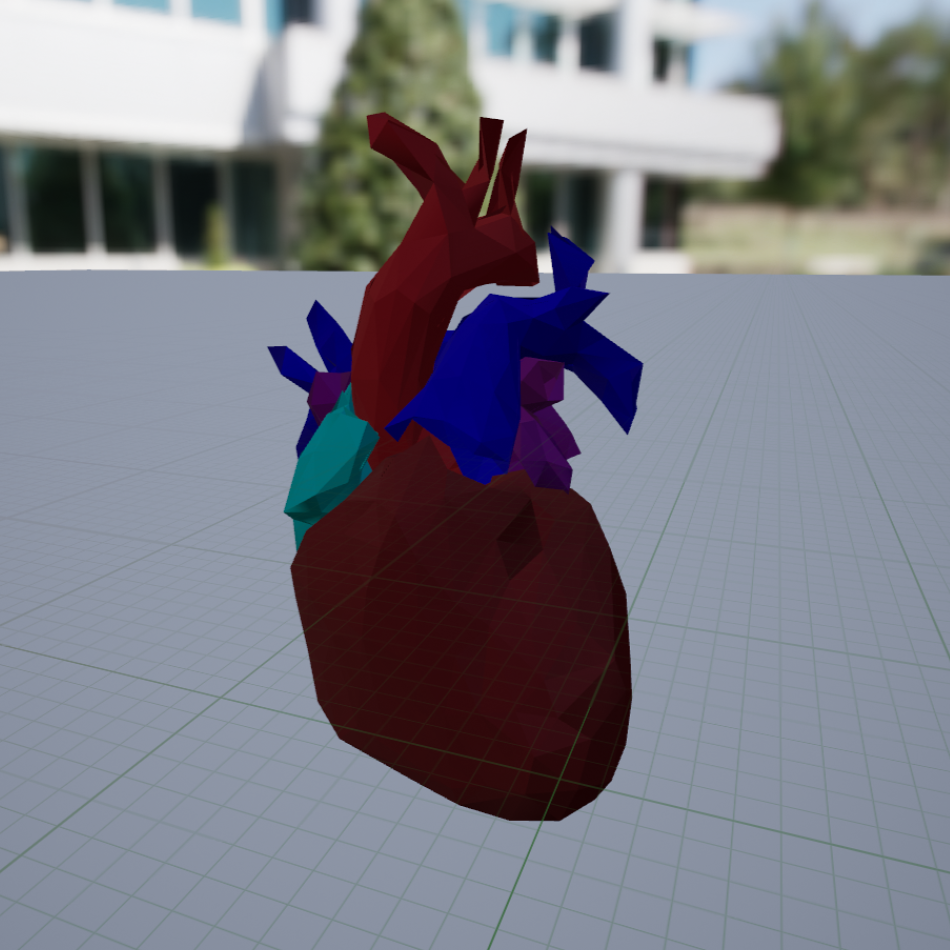
\includegraphics[width=\linewidth]{vrScreenshot/lod3.png}
      \caption{2\%}
  \end{subfigure}
  \caption{LODs and their percentages of a model of 96.180 triangles}
  \label{fig:lods}
\end{figure}

\paragraph{Removing opacity:}
Opacity is one of the heaviest options in shading, so for reducing GPU overhead it will be removed.

\paragraph{Clever level design:}
When watching 3D animations or playing video games, we might assume that every environment is fully constructed with maximum detail.
This is not the case. For example, in this case study, it's unnecessary to build parts like the exterior of a building or create a second floor.
Similarly, distant mountains may appear to have realistic depth, but they are often floating in empty space and are not actually far away.
This approach prevents the engine from loading hidden models, which would otherwise waste resources.\\
For the same reason, shaders are applied only to one side of a triangle.
For example, shading the inner side of thick building walls is unnecessary and would only consume resources without adding to the visual quality.\\
These triks can been seen in Fig.[\ref{fig:design}]



\begin{figure}[ht]
  \centering
  \includegraphics[width =\textwidth]{./vrScreenshot/design.png}
  \caption{Exterior of buildings}
  \label{fig:design}
\end{figure}

\section{General performance}
\noindent
One of the primary requirements was for the application to run at 90 \ac{FPS} for optimal comfort, and this target was achieved. As shown in Fig.[\ref{fig:performance}],
the app maintains a stable 90 \ac{FPS}, with minor performance drops occurring mainly during rendering and manipulation of 3D models.\\
To minimize these performance drops further, reducing the polygon count of the 3D models may be necessary to lighten their GPU load.
Fig.[\ref{fig:performance}] also illustrates that the bottleneck lies with the GPU, which handles rendering and manipulation of the 3D models.

\begin{figure}[ht]
  \centering
  
\includegraphics[width =0.96\textwidth]{./vrScreenshot/performance.png}
  \caption{Performance graph}
  \label{fig:performance}
\end{figure}

\section{Parser performance}\noindent
The parser performance must be efficient enough to avoid making the user wait too long. Fortunately, there is a generous upper time limit, as the models need to be downloaded first.
Ideally, parser performance should be $O(n)$, however for cleaner code, we are using a function called \texttt{ParseIntoArrayLines}, which returns the file as an array of its rows.
According to the \ac{UE} documentation\footnote{\url{https://dev.epicgames.com/documentation/en-us/unreal-engine/API/Runtime/Core/Containers/FString/ParseIntoArrayLines?application_version=5.2}}, this function is expected to have $O(n^2)$ complexity in terms of allocation.
However, my results suggest this may not be accurate—likely due to processor cache compensating for access speed.

\paragraph{Banchmark}
Table Tab.[\ref{tab:banchmark}] presents benchmark results showing the parser performance alongside the network time required to download it.
The test was conducted using a developer build of the app with all functionalities enabled. The connection was Wi-Fi 5 (up to 866 Mbps), with the access point approximately 2 meters from the \ac{HMD}.
The router was connected to a 1 Gbps fiber line, providing ideal network conditions.
As shown, the time to download the model is the real bottleneck and in real-world conditions, however, the \ac{HMD} may not benefit from such optimal network connectivity.\\
Thus, we can conclude that the parser performance is adequate for these use cases.

\begin{table}
  \centering
  \begin{tblr}{
      colspec = {|l|l|l|l|l|},
      rows={valign=m},
      row{1}={font=\bfseries}
    }
    \hline
    Size&Vertices & Triangles & Parsing time avg & Dowload time avg\\ \hline
    188kB&1284&  2568 &0.013700s &   0.160968s \\ \hline %RCA.obj
    276kB&1856&  3704 &0.020405s&  0.198955s   \\ \hline %Steel.obj
    540kB&3590&7192&0.037820s&0.215038s\\ \hline %LSA.obj
    724kB&4768&9564&0.050700s&0.230261s\\ \hline % RSA.obj
    1.7MB&10968&  21968 &0.116693s&   0.324465s  \\ \hline %Sternum.obj
    6.2MB&38207&  77474 &0.412519s&0.732149s\\ \hline %Thorax.obj
    9.7MB&60333&  120774 &0.630291s&0.985465s\\ \hline %Esempio.obj
    11MB&62674&126376&0.670590s&1.120609s\\ \hline %heart.obj
  \end{tblr}
  \caption{Parser loading time}
  \label{tab:banchmark}
\end{table}